%%
%% This is file `sample-sigconf.tex',
%% generated with the docstrip utility.
%%
%% The original source files were:
%%
%% samples.dtx  (with options: `all,proceedings,bibtex,sigconf')
%% 
%% IMPORTANT NOTICE:
%% 
%% For the copyright see the source file.
%% 
%% Any modified versions of this file must be renamed
%% with new filenames distinct from sample-sigconf.tex.
%% 
%% For distribution of the original source see the terms
%% for copying and modification in the file samples.dtx.
%% 
%% This generated file may be distributed as long as the
%% original source files, as listed above, are part of the
%% same distribution. (The sources need not necessarily be
%% in the same archive or directory.)
%%
%%
%% Commands for TeXCount
%TC:macro \cite [option:text,text]
%TC:macro \citep [option:text,text]
%TC:macro \citet [option:text,text]
%TC:envir table 0 1
%TC:envir table* 0 1
%TC:envir tabular [ignore] word
%TC:envir displaymath 0 word
%TC:envir math 0 word
%TC:envir comment 0 0
%%
%% The first command in your LaTeX source must be the \documentclass
%% command.
%%
%% For submission and review of your manuscript please change the
%% command to \documentclass[manuscript, screen, review]{acmart}.
%%
%% When submitting camera ready or to TAPS, please change the command
%% to \documentclass[sigconf]{acmart} or whichever template is required
%% for your publication.
%%
%%
\documentclass[sigconf]{acmart}
%%
%% \BibTeX command to typeset BibTeX logo in the docs
\AtBeginDocument{%
  \providecommand\BibTeX{{%
    Bib\TeX}}}

%% Rights management information.  This information is sent to you
%% when you complete the rights form.  These commands have SAMPLE
%% values in them; it is your responsibility as an author to replace
%% the commands and values with those provided to you when you
%% complete the rights form.
\setcopyright{acmlicensed}
\copyrightyear{2025}
\acmYear{2025}
\acmDOI{XXXXXXX.XXXXXXX}
%% These commands are for a PROCEEDINGS abstract or paper.
\acmConference[ML '25]{Aprendizaje Automático}{June 03--05,
  2025}{Ciudad de México, México}
%%
%%  Uncomment \acmBooktitle if the title of the proceedings is different
%%  from ``Proceedings of ...''!
%%
%%\acmBooktitle{Woodstock '18: ACM Symposium on Neural Gaze Detection,
%%  June 03--05, 2018, Woodstock, NY}
\acmISBN{978-1-4503-XXXX-X/2025/06}


%%
%% Submission ID.
%% Use this when submitting an article to a sponsored event. You'll
%% receive a unique submission ID from the organizers
%% of the event, and this ID should be used as the parameter to this command.
%%\acmSubmissionID{123-A56-BU3}

%%
%% For managing citations, it is recommended to use bibliography
%% files in BibTeX format.
%%
%% You can then either use BibTeX with the ACM-Reference-Format style,
%% or BibLaTeX with the acmnumeric or acmauthoryear sytles, that include
%% support for advanced citation of software artefact from the
%% biblatex-software package, also separately available on CTAN.
%%
%% Look at the sample-*-biblatex.tex files for templates showcasing
%% the biblatex styles.
%%

%%
%% The majority of ACM publications use numbered citations and
%% references.  The command \citestyle{authoryear} switches to the
%% "author year" style.
%%
%% If you are preparing content for an event
%% sponsored by ACM SIGGRAPH, you must use the "author year" style of
%% citations and references.
%% Uncommenting
%% the next command will enable that style.
%%\citestyle{acmauthoryear}


%%
%% end of the preamble, start of the body of the document source.
\begin{document}

%%
%% The "title" command has an optional parameter,
%% allowing the author to define a "short title" to be used in page headers.
\title{F-VICE: Forecasting Velocity of Ice in Glaciers Using
  Machine Learning}

%%
%% The "author" command and its associated commands are used to define
%% the authors and their affiliations.
%% Of note is the shared affiliation of the first two authors, and the
%% "authornote" and "authornotemark" commands
%% used to denote shared contribution to the research.
\author{Rodrigo S. Cortez-Madrigal}
\authornote{Both authors contributed equally to this research.}
\email{rcortez@enesmorelia.unam.mx}
\orcid{1234-5678-9012}
\author{G.K.M. Tobin}
\authornotemark[1]
\affiliation{%
  \institution{Institute for Clarity in Documentation}
  \city{CDMX}
  \state{CDMX}
  \country{México}
}

\author{Luis Vicente Ruiz Hernandez}
\authornote{Both authors contributed equally to this research.}
\email{trovato@corporation.com}
\orcid{1234-5678-9012}
\author{G.K.M. Tobin}
\authornotemark[1]
\affiliation{%
  \institution{Institute for Clarity in Documentation}
  \city{CDMX}
  \state{CDMX}
  \country{México}
}

%%
%% By default, the full list of authors will be used in the page
%% headers. Often, this list is too long, and will overlap
%% other information printed in the page headers. This command allows
%% the author to define a more concise list
%% of authors' names for this purpose.
%\renewcommand{\shortauthors}{Trovato et al.}

%%
%% The abstract is a short summary of the work to be presented in the
%% article.
\begin{abstract}
  El deshielo de los glaciares es un fenómeno natural
  que ha aumentado en las últimas décadas debido al cambio climático.
  Este proceso tiene un impacto significativo en el nivel del mar y en los ecosistemas locales.  
  En este trabajo, proponemos un enfoque basado en aprendizaje automático para predecir la serie de tiempo de la velocidad de deshielo de los glaciares. 
  Utilizamos un conjunto de datos del proyecto $ITS_LIVE$ del Jet Propulsion Laboratory de la NASA, que a partir de imágenes satelitales, proporciona información sobre la velocidad de deshielo de los glaciares.
  Finalmente comparamos los resultados de distintos modelos de aprendizaje automático y discutimos los resultados obtenidos.
\end{abstract}

%%
%% Keywords. The author(s) should pick words that accurately describe
%% the work being presented. Separate the keywords with commas.
\keywords{Deshielo, Glaciares, Aprendizaje Automático, Predicción, Cambio Climático}
%% A "teaser" image appears between the author and affiliation
%% information and the body of the document, and typically spans the
%% page.
\begin{teaserfigure}
  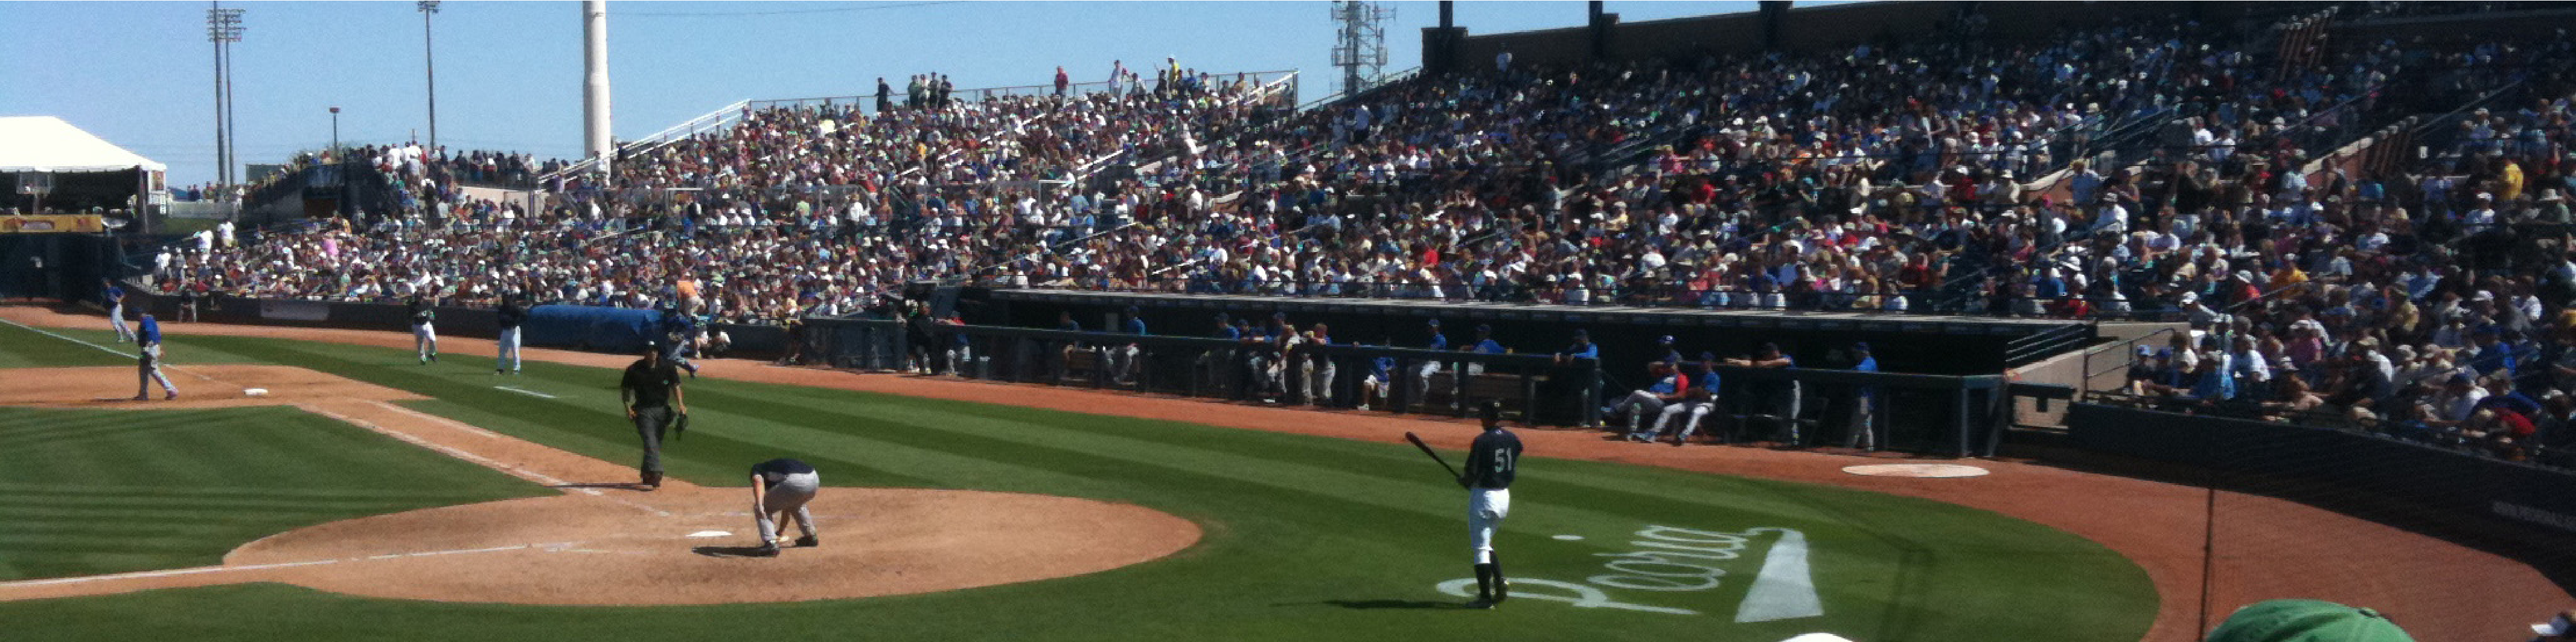
\includegraphics[width=\textwidth]{sampleteaser}
  \caption{Seattle Mariners at Spring Training, 2010.}
  \Description{Enjoying the baseball game from the third-base
  seats. Ichiro Suzuki preparing to bat.}
  \label{fig:teaser}
\end{teaserfigure}

\received{20 February 2025}
%\received[revised]{12 March 2025}
%\received[accepted]{5 June 2025}

%%
%% This command processes the author and affiliation and title
%% information and builds the first part of the formatted document.
\maketitle

\section{Introduction}

La predicción de series de tiempo es una tarea importante en el
ámbito del aprendizaje automático y la ciencia de datos. Desde la
predicción de precios de acciones hasta la predicción del clima, las
series de tiempo son una herramienta valiosa para la toma de decisiones
y la planificación. En este trabajo, nos enfocamos en la predicción de
la velocidad de deshielo de los glaciares, un fenómeno natural que ha
aumentado en las últimas décadas debido al cambio climático. 

ACM's consolidated article template, introduced in 2017, provides a
consistent \LaTeX\ style for use across ACM publications, and
incorporates accessibility and metadata-extraction functionality
necessary for future Digital Library endeavors. Numerous ACM and
SIG-specific \LaTeX\ templates have been examined, and their unique
features incorporated into this single new template.

If you are new to publishing with ACM, this document is a valuable
guide to the process of preparing your work for publication. If you
have published with ACM before, this document provides insight and
instruction into more recent changes to the article template.

The ``\verb|acmart|'' document class can be used to prepare articles
for any ACM publication --- conference or journal, and for any stage
of publication, from review to final ``camera-ready'' copy, to the
author's own version, with {\itshape very} few changes to the source.

\section{Antecedentes}

Distintos estudios han demostrado que el deshielo de los glaciares
es un fenómeno natural que ha aumentado en las últimas décadas debido
al cambio climático. Este proceso tiene un impacto significativo en
el nivel del mar y en los ecosistemas locales. Por lo tanto, es
importante contar con herramientas que permitan predecir la velocidad
de deshielo de los glaciares para poder tomar decisiones informadas
y planificar acciones para mitigar los efectos del cambio climático.


As noted in the introduction, the ``\verb|acmart|'' document class can
be used to prepare many different kinds of documentation --- a
double-anonymous initial submission of a full-length technical paper, a
two-page SIGGRAPH Emerging Technologies abstract, a ``camera-ready''
journal article, a SIGCHI Extended Abstract, and more --- all by
selecting the appropriate {\itshape template style} and {\itshape
  template parameters}.

This document will explain the major features of the document
class. For further information, the {\itshape \LaTeX\ User's Guide} is
available from
\url{https://www.acm.org/publications/proceedings-template}.

\subsection{Template Styles}

The primary parameter given to the ``\verb|acmart|'' document class is
the {\itshape template style} which corresponds to the kind of publication
or SIG publishing the work. This parameter is enclosed in square
brackets and is a part of the {\verb|documentclass|} command:
\begin{verbatim}
  \documentclass[STYLE]{acmart}
\end{verbatim}

Journals use one of three template styles. All but three ACM journals
use the {\verb|acmsmall|} template style:
\begin{itemize}
\item {\texttt{acmsmall}}: The default journal template style.
\item {\texttt{acmlarge}}: Used by JOCCH and TAP.
\item {\texttt{acmtog}}: Used by TOG.
\end{itemize}

The majority of conference proceedings documentation will use the {\verb|acmconf|} template style.
\begin{itemize}
\item {\texttt{sigconf}}: The default proceedings template style.
\item{\texttt{sigchi}}: Used for SIGCHI conference articles.
\item{\texttt{sigplan}}: Used for SIGPLAN conference articles.
\end{itemize}

\subsection{Template Parameters}

In addition to specifying the {\itshape template style} to be used in
formatting your work, there are a number of {\itshape template parameters}
which modify some part of the applied template style. A complete list
of these parameters can be found in the {\itshape \LaTeX\ User's Guide.}

Frequently-used parameters, or combinations of parameters, include:
\begin{itemize}
\item {\texttt{anonymous,review}}: Suitable for a ``double-anonymous''
  conference submission. Anonymizes the work and includes line
  numbers. Use with the \texttt{\string\acmSubmissionID} command to print the
  submission's unique ID on each page of the work.
\item{\texttt{authorversion}}: Produces a version of the work suitable
  for posting by the author.
\item{\texttt{screen}}: Produces colored hyperlinks.
\end{itemize}

This document uses the following string as the first command in the
source file:
\begin{verbatim}
\documentclass[sigconf]{acmart}
\end{verbatim}

\section{Metodología}

Modifying the template --- including but not limited to: adjusting
margins, typeface sizes, line spacing, paragraph and list definitions,
and the use of the \verb|\vspace| command to manually adjust the
vertical spacing between elements of your work --- is not allowed.

{\bfseries Your document will be returned to you for revision if
  modifications are discovered.}

\section{Experimentos y Resultados}

The ``\verb|acmart|'' document class requires the use of the
``Libertine'' typeface family. Your \TeX\ installation should include
this set of packages. Please do not substitute other typefaces. The
``\verb|lmodern|'' and ``\verb|ltimes|'' packages should not be used,
as they will override the built-in typeface families.

\section{Conclusiones}

The title of your work should use capital letters appropriately -
\url{https://capitalizemytitle.com/} has useful rules for
capitalization. Use the {\verb|title|} command to define the title of
your work. If your work has a subtitle, define it with the
{\verb|subtitle|} command.  Do not insert line breaks in your title.

If your title is lengthy, you must define a short version to be used
in the page headers, to prevent overlapping text. The \verb|title|
command has a ``short title'' parameter:
\begin{verbatim}
  \title[short title]{full title}
\end{verbatim}

\end{document}
\endinput
%%
%% End of file `sample-sigconf.tex'.
